\documentclass[12pt]{report}
\usepackage[utf8]{inputenc}
\usepackage[T1]{fontenc}
\usepackage[portuguese, brazil, english]{babel}
\usepackage{graphics}
\usepackage{url}
\usepackage{lipsum}
\usepackage{graphicx}
\usepackage{geometry}
\usepackage{amssymb}
\usepackage{float}
\usepackage{verbatim} 
\usepackage{amsmath} 
\usepackage{amsfonts}
\usepackage{amssymb}
\usepackage{lmodern}
\usepackage[portuguese,ruled,lined]{algorithm2e}
\usepackage{algorithmic}
\usepackage{caption}
\usepackage{subcaption}
\usepackage{indentfirst}
\usepackage{mathrsfs,amsmath}
\usepackage{amstext}
\usepackage{hyperref}
\usepackage{setspace}
\usepackage[refpage]{nomencl}
\usepackage{nomencl}
% \usepackage[alf,abnt-etal-cite=2,abnt-etal-list=0,abnt-etal-text=it,versalete,bibjustif]{abntex2cite}
\usepackage[alf]{abntex2cite}
\usepackage{tikz}
\usepackage{amsmath}
\usepackage{pgfplots}
\pgfplotsset{compat=1.13}
\usepackage{epstopdf}
\usepackage{datetime}
\usepackage{pgfplots}
%\usepackage[acronym]{glossaries}
%\usepackage{glossaries}
\usepackage{acro}
\usepackage[toc,titletoc]{appendix}
\usepackage{listings}
\usepackage{color}
\definecolor{dkgreen}{rgb}{0,0.6,0}
\definecolor{gray}{rgb}{0.5,0.5,0.5}
\definecolor{mauve}{rgb}{0.58,0,0.82}
\lstset{
  frame=tb,
  language=c++,
  aboveskip=3mm,
  belowskip=3mm,
  showstringspaces=false,
  columns=flexible,
  basicstyle={\small\ttfamily},
  numbers=none,
  numberstyle=\tiny\color{gray},
  keywordstyle=\color{blue},
  commentstyle=\color{dkgreen},
  stringstyle=\color{mauve},
  breaklines=true,
  breakatwhitespace=true,
  tabsize=3
}
%\usepackage[acronym]{glossaries}
%\usepackage{longtable}
% probably a good idea for the nomenclature entries:
%\acsetup{first-style=short}
% class `abbrev': abbreviations:
%\DeclareAcronym{ny}{
%  short = NY ,
%  long  = New York ,
%  class = abbrev
%}
%\DeclareAcronym{la}{
%  short = LA ,
%  long  = Los Angeles ,
%  class = abbrev
%}
%\enableregime[utf]

\hypersetup{
    %bookmarks=true,         % show bookmarks bar?
    unicode=false,          % non-Latin characters in Acrobat’s bookmarks
    pdftoolbar=true,        % show Acrobat’s toolbar?
    pdfmenubar=true,        % show Acrobat’s menu?
    pdffitwindow=false,     % window fit to page when opened
    pdfstartview={FitH},    % fits the width of the page to the window
    pdftitle={My title},    % title
    pdfauthor={Author},     % author
    pdfsubject={Subject},   % subject of the document
    pdfcreator={Creator},   % creator of the document
    pdfproducer={Producer}, % producer of the document
    pdfkeywords={keyword1, key2, key3}, % list of keywords
    pdfnewwindow=true,      % links in new PDF window
    colorlinks=true,       % false: boxed links; true: colored links
    linkcolor=blue,          % color of internal links (change box color with linkbordercolor)
    citecolor=blue,        % color of links to bibliography
    filecolor=magenta,      % color of file links
    urlcolor=blue           % color of external links
}
\geometry{left=2.5cm, top=2cm, bottom=2.5cm, right=2cm}
\newcommand{\euler}{\textit{e}}
\newcommand{\complexSymbol}{\textit{j}}
\setstretch{1.5}

\hfuzz=30pt
%\vfuzz=20pt
\hbadness=2000
\vbadness=\maxdimen

\def\worktitle{Desenvolvimento de um {\it drum pad} usando visão artificial}
\def\workauthor{Luciano Rodrigues Lucio Neto}
\def\workadvisor{Agostinho de Medeiros Brito Júnior}

\usepackage{afterpage}

\newcommand\blankpage{%
    \null
    \thispagestyle{empty}%
    \addtocounter{page}{-1}%
    \newpage}


\acsetup{first-style=short}

% Exemplos de acrônimos, se necessários...
% class `abbrev': abbreviations:
\DeclareAcronym{DFT}{
  short = DFT ,
  long  = \textit{Discrete Fourier Transform} ,
  class = abbrev
}
\DeclareAcronym{IDFT}{
  short = IDFT ,
  long  = \textit{Inverse Fourier Transform} ,
  class = abbrev
}
\DeclareAcronym{FFT}{
  short = FFT ,
  long  = \textit{Fast Fourier Transform} ,
  class = abbrev
}

\DeclareAcronym{IFFT}{
  short = IFFT ,
  long  = \textit{Inverse Fast Fourier Transform} ,
  class = abbrev
}
\DeclareAcronym{2D DFT}{
  short = 2D DFT ,
  long  = \textit{Two-Dimensional Discrete Fourier Transform} ,
  class = abbrev
}

\begin{filecontents}{data.dat}
 n   xn
 1    1
 3    1
 4    3
 6    3 
 7    5
 9    8
 11   8
 12   3
 14   3
 15   5
 17   10
 19   10
 20   3
 22   3
 23   5
 25   6
 27   6
 28   5
 30   5
 31   3
\end{filecontents}

\providecommand{\keywords}[1]{\textbf{\textit{Keywords: }} #1}
\providecommand{\palavrasChaves}[1]{\textbf{\textit{Palavras-chaves: }} #1}

\newdateformat{monthyeardate}{%
  \monthname[\THEMONTH], \THEYEAR}
%%%%%%%%%%%%%%%%%%%%%%%%%%%%%%%%%%%%%%%%%%%%%%%%%%%%%%%%%%%%%
\newcommand{\GG}[1]{}

\begin{document}

\selectlanguage{brazil}
\begin{titlepage}

  \centering
  {\normalsize \workauthor \par}
  %\includegraphics[width=0.15\textwidth]{example-image-1x1}\par\vspace{1cm}
  %{\scshape\LARGE Universidade Federal do Rio Grande do Norte \par}
  \vfill
  {\Large\bfseries \worktitle \par}
  \vfill

% Bottom of the page

  {\normalsize Brasil\par}
  {\normalsize \monthyeardate\today}
\end{titlepage}

\begin{titlepage}
  \centering
  {\small Universidade Federal do Rio Grande do Norte - UFRN \par}
  {\small Coordenação do Curso de Engenharia de Computação e Automação - DCA \par}
  {\small Graduação em Engenharia de Computação \par}
  \vfill

  {\normalsize \workauthor\par}
  %\includegraphics[width=0.15\textwidth]{example-image-1x1}\par\vspace{1cm}
  %{\scshape\LARGE Universidade Federal do Rio Grande do Norte \par}
  \vfill
  \centering
  {\Large\bfseries \par}
  \vfill

  \begin{flushright}  
  \begin{minipage}{15em}  
  \setstretch{1.0}
    Trabalho de Conclusão de Curso Submetido à Coordenação do Curso de Engenharia de Computação e Automação do Centro de Tecnologia da Universidade Federal do Rio Grande do Norte, como parte dos requisitos necessários para a obtenção do grau de Engenheiro de Computação.
  \end{minipage}
  \end{flushright}  
  \vfill
  
  
  \normalsize
  \centering
  {\normalsize Orientador: Agostinho de Medeiros Brito Júnior \par}
  \vfill
% Bottom of the page
  {\normalsize Brasil\par}
  {\normalsize \monthyeardate\today}
\end{titlepage}

\pagenumbering{gobble}% Remove page numbers (and reset to 1)

%%%%%% AGRADECIMENTOS %%%%%%

\chapter*{\centerline{Agradecimentos}}

Gostaria de agradecer a meus amigos, minha família, colegas e professores, mas, principalmente a minha mãe, Amanda Nazaré Pinho do Rosário, e a minha avó, Osmarina Pinho do Rosário, por todo o apoio e ajuda dados no âmbito familiar e ao professor orientador deste trabalho, Agostinho de Medeiros Brito Júnior, por todo o apoio, atenção e ajuda dados na esfera acadêmica, ajudando, inclusive, com a codificação em si e com soluções para problemas físicos, durante o desenvolvimento deste projeto.

Também gostaria de agradecer especialmente meus amigos Jadiel Azevedo, Jean Felipe Dantas, Matheus Lopes e Marcella Cavalcanti, os quais se envolveram ativamente com o processo de desenvolvimento do software dando ideias e ajudando com o algoritmo e com solução de problemas.

Sem esses grupos e pessoas específicas, o projeto não teria sido desenvolvido da maneira que foi e todos foram de suma importância para o término deste trabalho.

Muito obrigado a todos.

\newpage

%%%%%% RESUMO %%%%%%

\begin{abstract}
  Apresenta o desenvolvimento de um {\it drum pad} usando visão
  artificial capaz de controlar sintetizadores musicais virtuais
  criando uma sequência de notas musicais em repetição. Instrumentos
  assim são muito usados por músicos amadores que precisam criar
  acompanhamentos de bateria ou baixo para suas composições e não
  dispõem de músicos auxiliares para fazê-lo. A ferramenta criada
  permite que, usando apenas uma {\it webcam}, uma folha de papel e software
  livre, um músico amador seja capaz de criar efeitos semelhantes aos
  de um drum pad físico desenhando em uma folha de papel.
  \\
  \palavrasChaves{Drum pad, sequenciador, controlador midi, OpenCV,
    Visão artificial}
\end{abstract}

\newpage

%%%%%% RESUMO EM INGLÊS %%%%%%
\selectlanguage{english}

\begin{abstract}
  {\it Introduces the development of a drum pad utilizing artificial vision capabçe of controling virtual synthesizers creating a sequence of musical notes on loop. Instruments like these are commonly used by amateur musicians artist who need to generate drums or bass support to their compositions and couldn't find other musicians to support it. The developed tool allows that with only a webcam, one paper sheet and open source software, an amateur musician artist can be able to replicate simmilar effects of a physical drum pad while drawing over a paper sheet.}
  \keywords{Drum pad, sequencer, midi controller, OpenCV, artificial vision}

\end{abstract}

\newpage

\selectlanguage{brazil}

%%%%%% LISTA DE FIGURAS %%%%%%

\listoffigures

\newpage

%%%%%% LISTA DE ABREVIAÇÕES %%%%%%

%{\centering
%\printacronyms[include-classes=abbrev,name=Abreviações]
%}
\tableofcontents

%\makenomenclature
%\makeglossaries

%\newglossaryentry{DFT}{%
%name={DFT},%
%description={antigeen-presenterende cel}%
%}


\newpage

%%%%%% INÍCIO DO TEXTO %%%%%%

\pagenumbering{arabic}

\chapter{Introdução}
\label{cha:introducao}

Um {\it drum pad} é um periférico utilizados por músicos e entusiastas
de música eletrônica de diferentes formas. Sua principal função é
reproduzir sons escolhidos pelo usuário ao apertar de botões de sua
interface e, dada a simplicidade de uso, é muito popular na comunidade
de músicos sendo eles profissionais ou amadores.

{\it Drum pads} também são utilizados como uma forma de se programar
uma sequência de sons que serão reproduzidos em um intervalos de tempo
específico, servindo como acompanhamento musical com diversas
aplicações, sejam elas para guiar um músico, acompanhar o ritmo com
alguma percussão ou até reproduzir detalhes específicos que o usuário
pode não conseguir no momento correto.

Apesar de ser um periférico de fácil utilização e de rápida
adaptabilidade, ainda depende da capacidade do usuário em reproduzir
as notas no tempo correto e principalmente da capacidade que o usuário
tem em investir num equipamento do tipo, com investimentos que variam
de cerca de 50 dólares, podendo chegar a mais de 600 dólares,
dependendo do seu tamanho, sua funções, características, inovações e
acabamento.

A proposta do projeto apresentado neste trabalho de conclusão de curso
é facilitar a programação de uma sequência de sons que um usuário
venha querer utilizar. Com apenas uma webcam de baixo custo, uma folha
de papel e um programa de computador que utiliza conceitos de visão
artificial, o usuário é capaz de programar, de forma interativa, uma
sequência de sons em um sintetizador midi. A sequência será
reproduzida em um tempo determinado a partir de marcações feitas na
folha e sem depender, por exemplo, de suas próprias habilidades
rítmicas.

No capítulo um será apresentado o modelo utilizado como referência
para se utilizar o software apresentado neste trabalho, no capítulo
seguinte o algoritmo que o software utiliza para reproduzir sons de
acordo com o modelo. O capítulo seguinte explica conceitos básicos do
Protocolo MIDI utilizados no desenvolvimento do software. O capítulo
quatro apresenta os marcadores utilizados no modelo de folha de
papel, elementos cruciais para o funcionamento do software,, enquanto
o capítulo seguinte explica como, a partir desses marcadores, o
software aplica uma transformada de perspectiva da matriz da imagem
capturada pela câmera. No capítulo sete é explicado como se utilizar o
software. No próximo capítulo estão conceitos da biblioteca RtMidi,
utilizada para haver comunicação midi a partir do protocolo
apresentado no capítulo três, enquanto os próximos dois capítulos
discorrem, respectivamente, sobre resultados do software e conclusões
tiradas ao final do desenvolvimento do projeto.

\chapter{O padrão MIDI}
\label{cha:midi}

O Protocolo MIDI \cite{midi} é o padrão de comunicação em tempo real
entre controladores e sintetizadores de sons existentes no mercado e
está presente em uma grande quantidade de instrumentos musicais
eletrônicos disponíveis no mercado. Ele define padrões de {\it
  hardware} e de {\it software} que estabelecem como dispositivos MIDI
devem ser implementados de forma a se comunicarem entre si.

Um controlador MIDI é um dispositivo que não necessariamente produz
algum tipo de som. Sua tarefa é a de preparar a sequência de notas
musicais e suas durações e enviá-las ao sintetizador. Esse último, por
outro lado, possui capacidades de produzir sons conforme os códigos
MIDI recebidos de um sequenciador que é conectado a ele. Um controlador
MIDI, por exemplo, pode ser criado na forma de um teclado, controlando
um sintetizador que reproduz sons de uma bateria ou de voz humana.

O padrão MIDI estabelece um protocolo de comunicação universal, de
sorte que independe do fabricante do sintetizador ou sequenciador
quando estão conectados um ao outro. Apesar de bastante extenso e
complexo, apenas partes de sua especificação foram utilizadas no
projeto, de sorte que serão apresentados nesse documento as partes
pertinentes ao desenvolvimento da ferramenta. Em se tratando do
desenvolvimento de um software, apenas os detalhes envolvidos na
troca de mensagens nos moldes do protocolo são apresentadas.

A parte do protocolo que define os padrões de software consiste na
troca de "mensagens MIDI" entre o software ou hardware controlador,
que controla as notas e suas durações, e o software ou hardware
sintetizador, que sintetiza os sons.

Essas mensagens baseiam-se em um conjunto de um ou mais {\it bytes},
onde o primeiro {\it byte} se classifica como {\it STATUS byte}, o
qual define o tipo da mensagem, e é geralmente seguido por outros {\it
  bytes} chamados {\it DATA bytes}, os quais dão as características
desejadas para a mensagem.

Existem diversos tipos de mensagens mostradas na tabela \cite{tabela1} e de forma expandida na tabela \cite{tabela2}, extraídas
diretamente da {\it The MIDI Association} (\url{www.midi.org}),
principal portal com informações do protocolo MIDI. Para o
desenvolvimento do projeto foram utilizadas basicamente as mensagens
chamadas {\it Note ON} e {\it Note OFF}, que especificam quando uma
nota deve ser ativada e desativada.

Outras mensagens utilizadas, que são mensagens de
configuração do canal MIDI, são as mensagens {\it Control Change},
enviada para o sintetizador, no caso deste software, apenas na
inicialização do programa, a qual pode designar diversas ações
diferentes para o sintetizador. Porém, no software apresentado neste
trabalho, ela é utilizada apenas para controle de volume e a mensagem
{\it Program Change}, a qual seleciona o identificador do instrumento
que o sintetizador irá simular, enviada, neste software, assim como a
Control Change, apenas na sua inicialização.

As mensagens de ativação e desativação do som são compostas por um
conjunto de 3 {\it bytes} os quais são representados da seguinte
forma:
\begin{itemize}
  \item A mensagem {\it Note ON}:
  \begin{itemize}
    \item {\it Status byte}: 1001 nnnn
    \item {\it Data byte}: 0kkk kkkk
    \item {\it Data byte}: 0vvv vvvv
  \end{itemize}
  \item A mensagem {\it Note OFF}:
  \begin{itemize}
    \item {\it Status byte}: 1000 nnnn
    \item {\it Data byte}: 0kkk kkkk
    \item {\it Data byte}: 0vvv vvvv
  \end{itemize}
\end{itemize}

Onde os bits `nnnn` representam o canal que esta mensagem controlará,
variando entre 16 canais distintos, os bits `kkkkkkk` representam o
{\it pitch} que será reproduzido e os `vvvvvvv` representam a dinâmica
com a qual a nota será reproduzida que, em notação musical, são
representadas da seguinte maneira:

\begin{figure}[H]
  \centering
    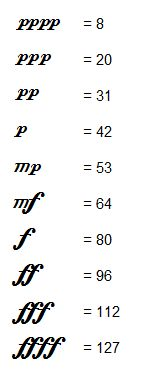
\includegraphics[width=0.2\textwidth]{imagens/nuance-velocity-table.jpg}
    \caption{Dinâmica em notação musical e seus respectivos valores
      para a mensagem {\it Note On}.}
  \label{fig:Velocidades em notação musical}
\end{figure}

Essa velocidade de reprodução, dependendo do tipo de instrumento
selecionado, também varia a dinâmica que o som é reproduzido como
quando uma nota de um piano é pressionada de forma brusca ou mais
suave.

Para as mensagens {\it Note OFF}, os {\it bits} nnnn e kkkkkkk
representam o mesmo da mensagem de ativação da nota, sendo diferente
apenas no terceiro {\it byte}, o vvvvvvv, que representa a velocidade
de liberação do som, ou seja, a suavização até ele ser desligado.

A mensagem de alteração de valores dos controladores é representada da seguinte maneira:
\begin{itemize}
  \item A mensagem {\it Control Change}:
  \begin{itemize}
    \item {\it Status byte}: 1000 nnnn
    \item {\it Data byte}: 0ccc cccc
    \item {\it Data byte}: 0vvv vvvv
  \end{itemize}
\end{itemize}

Nessa mensagem, os bits `nnnn` representam o canal para o qual a
mensagem será enviada, da mesma forma das mensagens de ativação e
desativação do som, `ccccccc` representa o controlador que terá o seu
valor alterado e vvvvvvv representa o valor que será atribuído para o
controlador. Os controladores controlados a partir dessas mensagens
podem variar entre 128 controladores destintos sendo eles os
seguintes:

\begin{figure}[H]
  \centering
    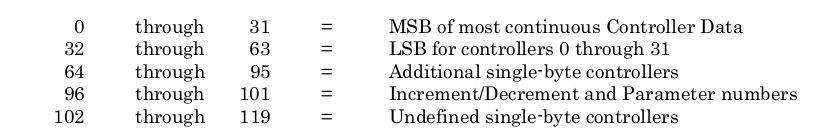
\includegraphics[width=\textwidth]{imagens/controladores.png}
    \caption{Controladores controlados a partir da mensagem {\it Control Change}}
  \label{fig:controladores}
\end{figure}

Com essa mensagem é possível variar em cada canal desde variáveis de
volume até variáveis de modulação e efeitos que caracterização como o
som será reproduzido pelo sintetizador.

A última mensagem utilizada no software, a  {\it Program  Change}, é
representada da seguinte maneira:
\begin{itemize}
  \item A mensagem {\it Control Change}:
  \begin{itemize}
    \item {\it Status byte}: 1100 nnnn
    \item {\it Data byte}: 0ppp pppp
  \end{itemize}
\end{itemize}

Onde `nnnn` representa o número do canal para o qual a mensagem será
enviada e `ppppppp` representa o identificador do instrumento que será
selecionado.

As mensagens que o software envia são sempre direcionadas ao canal um,
menos quando o modo de simulação de bateria está ativado. Quando esse
modo está ativado, o software envia as mensagens para o canal dez, o
qual, por padrão, possui um banco de simulação de instrumentos de
percussão ao invés de instrumentos melódicos nos sintetizadores midi.

O protocolo MIDI define muito mais coisas e comportamentos no processo
de comunicação entre máquinas ou {\it softwares}. Entretanto, estão
fora do escopo do trabalho, de sorte que os trechos mostrados nessa
seção são suficientes para compreender os 

\chapter{Os marcadores ArUco e seu papel na identificação do {\it drum
    pad}}
\label{cha:aruco}

A funcionalidade da ferramenta descrita nesse documento depende
intrinsecamente da região de interesse no {\it layout}. A
identificação dessas regiões normalmente é bem complicada, posto que o
usuário pode posicionar a câmera em locais que dificultam a extração
das zonas onde se encontram as informações úteis. O principal problema
encontrado é corrigir distorções de perspectiva. 

Para se identificar essa área de interesse da imagem, uma das soluções
mais simples é a utilização de marcadores fiduciais quadrados
binários. O principal benefício em se utilizar marcadores do tipo é de
se obter, a partir dos marcadores as pontos que determinam os limites
da região de interesse.

Marcadores fiduciais normalmente são fáceis e confiáveis para serem
detectados em uma cena. Introduzir seu uso para facilitar o processo
de identificação da região de interesse não prejudica o restante dos
elementos visuais da cena e ainda reduz a complexidade da tarefa de
detecção.

No desenvolvimento deste projeto foi escolhido o módulo ArUco da
biblioteca de visão artificial OpenCV para geração e identificação
desses marcadores.O módulo ArUco é baseado na biblioteca ArUco, uma
popular biblioteca utilizada para detecção de marcadores fiduciais
quadrados \cite{aruco2}, desenvolvida por Rafael Muñoz e Sérgio Garrido, em
aplicações de realidade aumentada.

A partir do módulo Aruco, pode-se gerar marcadores ArUco que consistem
em imagens quadradas compostas por uma larga borda da cor preta e
uma matriz binária intrínseca ao marcador, que determina seu
identificador. As bordas existem para facilitar a detecção do marcador
em uma imagem e a codificação da matriz binária para permitir a
detecção desse marcador com intuito de serem aplicadas outras técnicas
de visão artificial. Abaixo temos alguns exemplos de marcadores ArUco:

\begin{figure}[H]
  \centering
    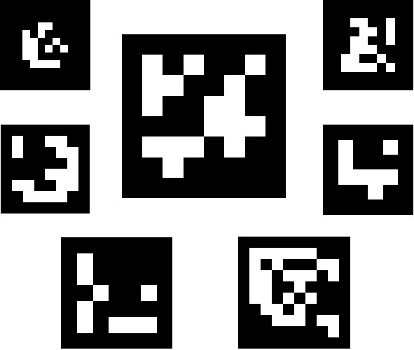
\includegraphics[width=0.2\textwidth]{imagens/markers.jpg}
    \caption{Exemplos de marcadores ArUco}
  \label{fig:arucoMarkers}
\end{figure}

Para a geração desses marcadores utilizando o código fornecido nos
exemplos da utilização da biblioteca na sua documentação
\cite{opencv}, é necessário informar o identificador do marcador e um
dicionário - dentre dezesseis diferentes - no qual o marcador está
presente. Opcionalmente, é possível se informar o número de bits na
borda do marcador, gerando uma borda maior ou menor, e o tamanho do
marcador, em pixels. O exemplo abaixo é um marcador criado a partir
desse código utilizando, como parâmetros de entrada, dois bits
dedicados para borda, dicionário \texttt{DICT\_4X4\_100},
identificador 10 e um tamanho de 50x50 pixels.

\begin{figure}[H]
  \centering
    
\includegraphics[width=0.15\textwidth]{imagens/marker.png}
    \caption{Marcador de identificador 10 presente no dicionário \texttt{DICT\_4X4\_100}}
  \label{fig:markers210}
\end{figure}

Para o software desenvolvido neste trabalho, os marcadores utilizados
foram os de identificadores 1, 2, 3 e 4 do dicionário
\texttt{DICT\_4X4\_250}, os quais podem ser vistos abaixo com mais
clareza:

\begin{figure}[H]
  \centering
  \begin{subfigure}{0.4\textwidth}
    \centering
    
\includegraphics[width=0.3\textwidth]{imagens/4x4_1000-1.png}
    \caption{Marcador do canto superior esquerdo.}
    \label{fig:TOPLEFT}
  \end{subfigure}
  %
  \begin{subfigure}{0.4\textwidth}
    \centering
    
\includegraphics[width=0.3\textwidth]{imagens/4x4_1000-2.png}
    \caption{Marcador do canto superior direito.}
    \label{fig:TOPRIGHT}
  \end{subfigure}
  %
  \begin{subfigure}{0.4\textwidth}
    \centering
    
\includegraphics[width=0.3\textwidth]{imagens/4x4_1000-3.png}
    \caption{Marcador do canto inferior esquerdo.}
    \label{fig:BOTTOMLEFT}
  \end{subfigure}
  %
  \begin{subfigure}{0.4\textwidth}
    \centering
    
\includegraphics[width=0.3\textwidth]{imagens/4x4_1000-4.png}
    \caption{Marcador do canto inferior esquerdo.}
    \label{fig:BOTTOMRIGHT}
  \end{subfigure}
\end{figure}

Já para detecção desses marcadores, utilizando a biblioteca de visão
computacional OpenCV, é possível utilizar a função {\it
  detecMarkers()}, a qual recebe como parâmetros a imagem de origem, o
dicionário ao qual as marcas utilizadas pertencem, um vetor para
armazenamento dos cantos dos marcadores, um vetor para armazenamento
dos identificadores dos marcadores, um objeto da classe {\it
  DetectorParameters} e um vetor para armazenamento das imagens
rejeitadas, ou seja, que foram classificadas como marcadores em algum
ponto do algoritmo, porém descartadas num segundo momento pelo
algoritmo da função.

O objeto da classe {\it DetectorParameters} tem valores padrão
atribuídos a ele pelo construtor da classe, porém, se for necessário,
é possível atribuir outros valores para os atributos do objeto, a fim
de alterar a forma que o algoritmo faz essa detecção. Os passos
seguidos, pelo algoritmo da função, para detecção das imagens são os
seguinte: primeiramente é aplicado um {\it thresholding} adaptativo na
imagem de origem, ou seja, um filtro com valores de limiar
definidos. Após isso, há uma filtragem dos contornos presentes na
imagem resultante do primeiro passo, que detectará os contornos
presentes na imagem, porém nem todos os contornos são considerados
marcadores.

Os contornos são filtrados em passos intermediários, os quais
descartam contornos que são considerados marcadores a fim de otimizar
o desempenho da detecção. Com os contornos e candidatos a marcadores
detectados, o algoritmo verifica se esses candidatos realmente são
marcadores ou não fazendo uma extração dos bits presentes em cada
candidato.

Na documentação é possível visualizar como a extração dos bits é
feita: primeiramente é feita uma transformada de perspectiva em cima
do candidato, a fim de remover qualquer distorção de perspectiva
indesejada, e o resultado é filtrado com o limiar de Otsu, a fim de
diferenciar pixels pretos e branco, como é mostrado na figura abaixo:

\begin{figure}[H]
  \centering
    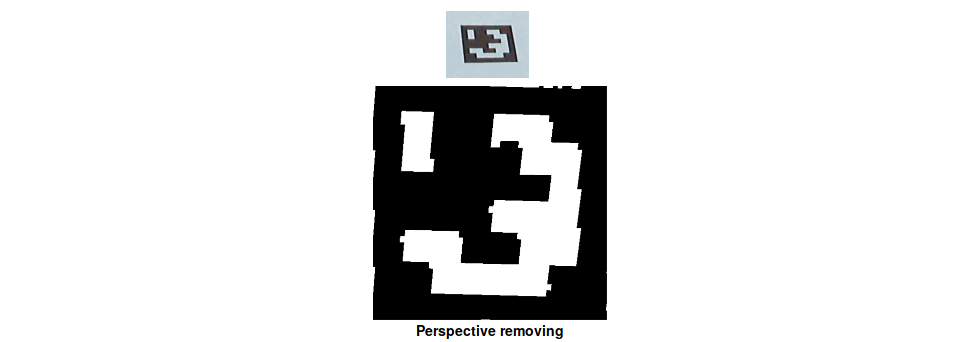
\includegraphics[width=0.7\textwidth]{imagens/bitsextraction.png}
    \caption{Remoção de perspectiva para detecção de marcador}
  \label{fig:bitsextraction}
\end{figure}

O próximo passo seguido pelo algoritmo é dividir a imagem em uma área
quadriculada, onde, em cada célula dessa área, há uma contagem de
pixels brancos e pretos, a fim de determinar se aquela célula é branca
ou preta.

\begin{figure}[H]
  \centering
    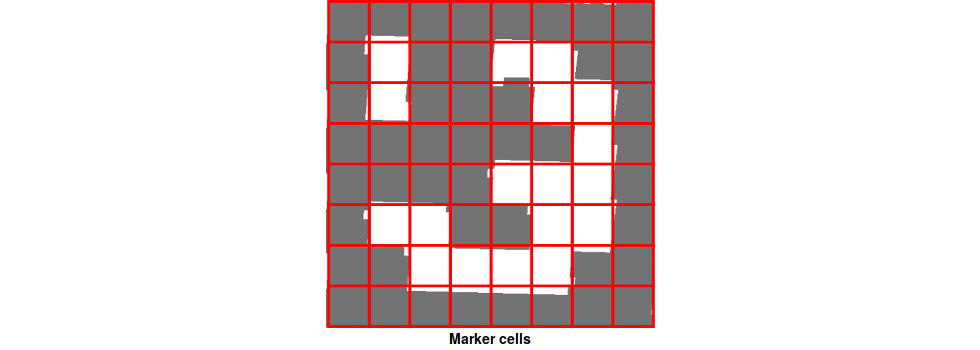
\includegraphics[width=0.7\textwidth]{imagens/bits2.png}
    \caption{Divisão em {\it grid}}
  \label{fig:bits2}
\end{figure}

Esse processo de contagem de pixels pretos e brancos pode ser
representado pela imagem abaixo. Nesse passo, são ignorados alguns
pixels da imagem a fim de otimizar o processo de contagem dos pixels.

\begin{figure}[H]
  \centering
    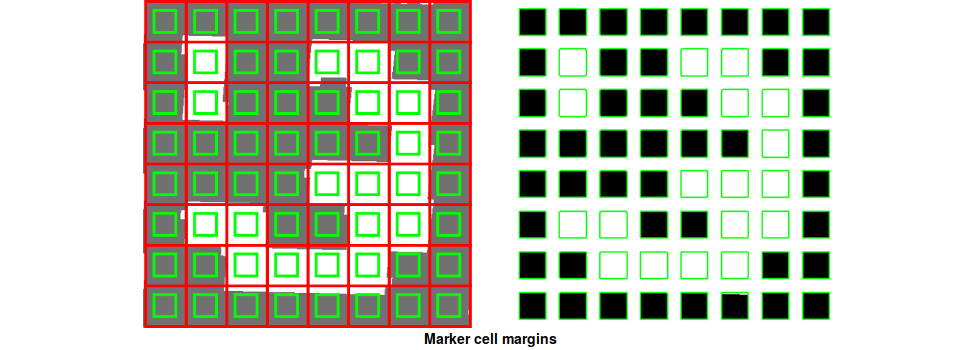
\includegraphics[width=0.7\textwidth]{imagens/bits3.png}
    \caption{Processo de ignorar alguns pixels para identificação do marcador}
  \label{fig:bits3}
\end{figure}

Após todos os passos do algoritmo de detecção de marcadores, é
possível obter-se os identificadores dos marcadores presentes na
imagem original, os seus quatro cantos, e os contornos dos objetos
rejeitados no processo intermediário no passo de detecção de contornos.

Com essa detecção rápida e precisa feita pela biblioteca OpenCV, foram
escolhidos quatro identificadores que simbolizam os cantos da folha
modelo. Após decodificar os quatro marcadores o software identifica as
coordenadas dos limites da região de interesse onde está a tabela para
marcação de notas e tempos.

Com a área de interesse adquirida, é aplicada uma transformação de
perspectiva nessa nova imagem a fim de desprezar distorções causadas
pelo posicionamento da câmera. A imagem produzida é uma versão
corrigida e sem distorções da tabela. Assim, fica fácil para o usuário
posicionar a câmera sem muita preocupação com ajustes finos de
posicionamento. 

Outra forma de identificação que foi testada no projeto foi por cores
em círculos coloridos posicionados no canto da folha. Devido à
diversas variáveis de ambiente, essas cores poderiam variar de usuário
para usuário, local para local, câmera para câmera entre outros, o que
tornava necessária a marcação das cores ser feita manualmente pelo
usuário com o propósito de haver um cálculo da média da cores dos
círculos para sua identificação e, devido a essa inconsistência ao
utilizar cores, a ideia foi descartada. O modelo anterior pode ser
visto abaixo:

\begin{figure}[H]
  \centering
    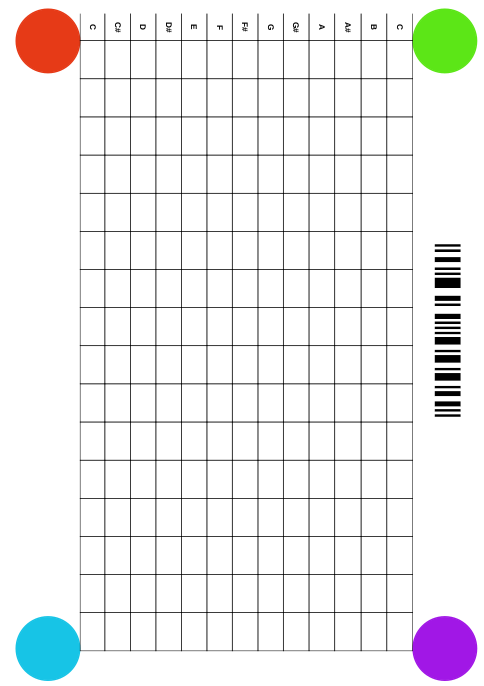
\includegraphics[angle=90,origin=c,width=0.5\textwidth]{imagens/circulos.png}
    \caption{Modelo com círculos}
  \label{fig:circulos}
\end{figure}

\chapter{{\it Drum pads} físicos e a construção de um equivalente
  virtual}
\label{cha:drum_pads}

Os equipamentos e programas de computador disponíveis no mercado que
serviram como referência para o desenvolvimento do software
apresentado neste trabalho podem ser chamados de {\it drum pads}, {\it
  sample pads} ou {\it sampling pads}. As principais diferenças entre
eles são que, nos {\it sample} ou {\it sampling pads}, diferentemente
dos {\it drum pads}, não há simulação apenas de instrumentos de
percussão, mas também aceitam sons customizados, ou {\it samples}, e
por esse motivo são bastante utilizados por DJ's.

Os preços dos equipamentos, nos casos mais baratos, variam na faixa
dos 50 ou 60 dólares podendo chegar, em casos de equipamentos
profissionais, a bem mais de 600 dólares. Já os programas disponíveis
principalmente para smartfones modernos, encontrados de graça podendo
chegar à faixa dos 30 dólares.

Devido à inviabilidade de serem testados equipamentos do tipo descritos
anteriormente por questões de preço e indisponibilidade em lojas
físicas, foram testados três aplicativos disponibilizados de forma
gratuita na {\it Play Store} da Google, disponível em smartfones com
o sistema operacional Android. Os softwares foram os {\it Electro
  Music Drum Pads} \cite{app1}, publicado pela {\it AppX Apps}, {\it
  Drum Pad Machine} - Crie música \cite{app2}, publicado pela {\it
  Easybrain}, e {\it Drum Pad 24 - Music Maker} \cite{app3}, publicado
por {\it Paul Lipnyagov}. Abaixo é possível visualizar os menus
principais de cada um dos três:

\begin{figure}[H]
  \centering
  \begin{subfigure}{0.4\textwidth}
    \centering
    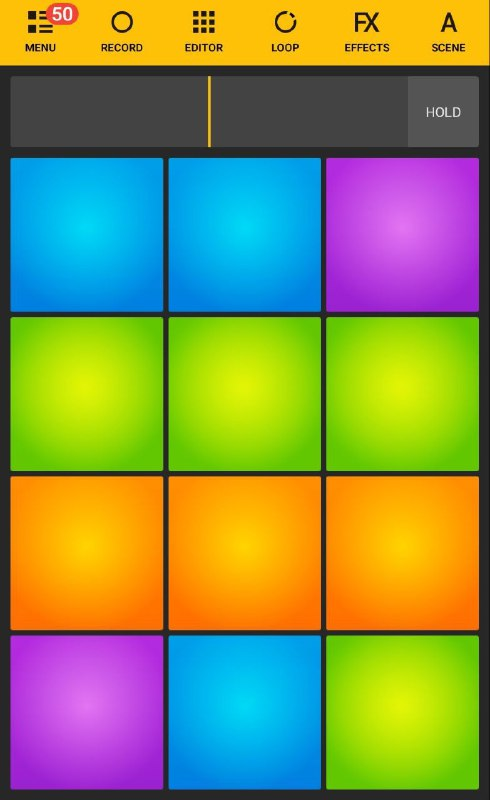
\includegraphics[width=0.4\textwidth]{imagens/drumpads24.jpeg}
    \caption{{\it Drum Pad 24 - Music Maker}}
    \label{fig:emdp}
  \end{subfigure}
  %
  \begin{subfigure}{0.4\textwidth}
    \centering
    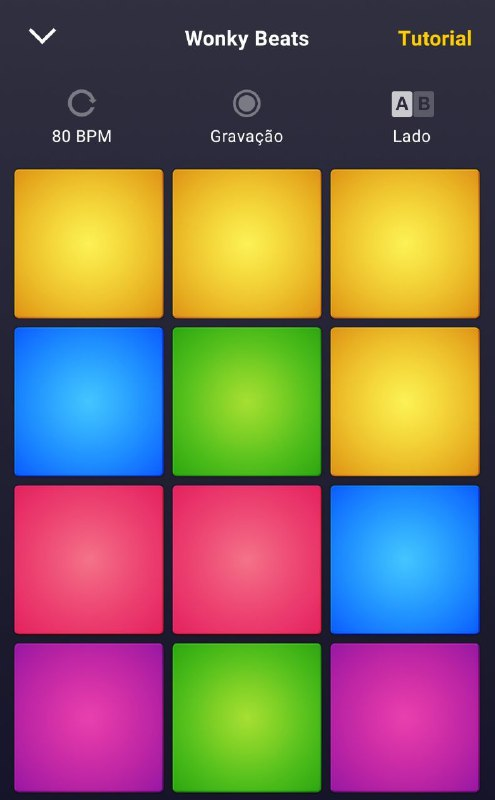
\includegraphics[width=0.4\textwidth]{imagens/dpm.jpeg}
    \caption{{\it Drum Pad Machine} - Crie música}
    \label{fig:dpm}
  \end{subfigure}
  %
  \begin{subfigure}{0.4\textwidth}
    \centering
    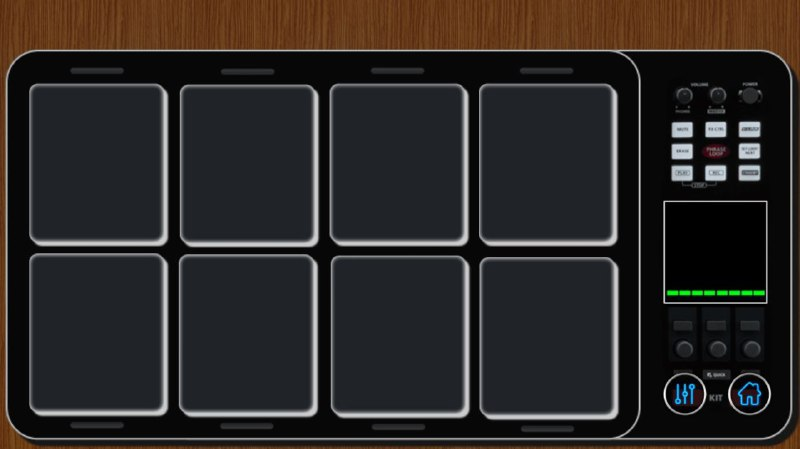
\includegraphics[width=0.6\textwidth]{imagens/emdp.jpeg}
    \caption{{\it Electro Music Drum Pads}}
    \label{fig:drumpads24}
  \end{subfigure}
\end{figure}

O aplicativo {\it Electro Music Drum Pads} é um {\it drum pad} e
apresenta apenas uma interface para reprodução dos sons ao toque dos
botões e uma outra interface para seleção de parâmetros de controle
para reprodução dos sons como volume e compressão, já os outros dois
analisados são {\it sample pads}. Ambos {\it Drum Pad Machine} - Crie
música e {\it Drum Pad 24 - Music Maker} apresentam diversos pacotes
de sons diferentes, sendo alguns gratuitos e outros pagos, com 24 sons
diferentes em cada. Também possuem funcionalidades para programação de
{\it loop} sendo um com 32 sons e outro com 24, gravação para
armazenando do áudio gravado na memória oferecida pelo dispositivo que
está executando o aplicativo e, no {\it Drum Pad 24 - Music Maker},
uma interface para controle de tom dos vinte e quatro sons. Apesar de
aparentemente mais completo, o aplicativo {\it Drum Pad 24 - Music
  Maker} peca principalmente na interface para programação de
repetições, apesar de ambos terem uma limitação de quantos sons podem
ser programados em sequência.

O software desenvolvido neste trabalho tem como objetivo simular a
função de programação de sequências desses aplicativos e, apesar das
limitações físicas, dá mais probabilidades para o usuário, tornando
mais livre a sua aplicação final, porém, por utilizar exclusivamente o
protocolo MIDI para comunicação com softwares sintetizadores MIDI, não
reproduz sons customizados, o que o torna um {\it drum pad} capaz de
aceitar, além de bancos de simulação de percussão, bancos de simulação
de instrumentos melódicos como piano, órgão, gaita, violão entre
diversos outros.

De acordo com pesquisas feitas, mas apesar de não testados, os
hardwares, principalmente os mais caros e mais profissionais, sempre
disponibilizam para o usuário um software próprio daquele hardware com
bancos de sons pré selecionados e, em alguns casos, com formatos
compatíveis com bancos disponíveis online para download, ou o próprio
hardware já possui um banco interno com sons pré selecionados. Além
disso, possuem interfaces de entrada e saída MIDI, o que torna
possível serem utilizados como controladores MIDI padrão.

Tendo em vista todas as possibilidades que os periféricos desse tipo
dão para o usuário, eles certamente são a escolha mais certa para
alguém que pretende utilizá-los de forma mais profissional, uma vez
que são extremamente completos, porém o investimento será compatível
com a qualidade do periférico e o software apresentado neste trabalho
com desenvolvido para ser uma opção para um usuário que, tendo uma
webcam, procura algo que solucione ao menos a questão de repetição de
sons em sequência, além de ter outras aplicações discorridas durante
os próximos capítulos deste documento.

\section{Construindo um {\it drum pad} virtual}

Assim como muitas aplicações que envolvam conceitos de visão
artificial, é necessário um ambiente controlado de onde se possa
extrair as informações necessárias para o funcionamento do programa de
computador. Para isso, foi necessária a criação de um {\it layout} com
elementos específicos que façam com que o ambiente seja bem
interpretado pelo programa.

\begin{figure}[H]
  \centering
  \includegraphics[angle=90,origin=c,width=0.5\textwidth]{imagens/modelo44.png}
  \caption{Modelo da folha com quatro notas por batida}
  \label{fig:modelo_}
\end{figure}

As principais características do {\it layout} para que haja a
interação com o programa de computador são os marcadores nos cantos da
folha e o código de barras.

Tendo em vista que, nesse modelo, sempre haverão 13 notas distintas
que podem ser reproduzidas (contempla apenas uma das oitavas de um
piano), o código de barras é utilizado para guardar a informação de
quantas notas o programa pode reproduzir e sua fórmula de compasso,
sem haver a necessidade do usuário especificá-las.

Não faria sentido o modelo ter, por exemplo, uma área quadriculada de
13x8 e o usuário configurar que o essa área tem uma distribuição
diferente da real ou uma fórmula de compasso que não corresponda ao
modelo. Além do código de barras, são utilizados marcadores nos cantos
da folha que, ao serem interpretados, mostram a imagem final que o
programa utilizará como fonte de interpretação.

\section{Transformação de Perspectiva para correção de distorções}
\label{sec:perspectiva}

Para o software interpretar a imagem de forma correta, seria
necessário que ela estivesse perfeitamente paralela à câmera, tornando
desconfortável a sua utilização. Uma maneira de solucionar esse
problema foi utilizar uma transformada de perspectiva, desprezando os
problemas gerados para imagens capturadas de posições que não sejam
paralelas à câmera que está capturando o ambiente.

Graças à biblioteca OpenCV, essa manipulação é de rápida e fácil
aplicação, precisando-se apenas de quatro pontos de referência na
imagem original e uma nova matriz imagem resultado.

A partir dos quatro pontos da imagem original, aplica-se a função {\it
  getPerspectiveTransform()}, que a partir da fórmula mostrada abaixo,
gera uma matriz de transformação de perspectiva 3x3:

\begin{equation}
  \begin{bmatrix}
    t{}_i x'{}_i \\
    t{}_i y'{}_i \\
    t{}_i
  \end{bmatrix} = MapMatrix \times
  \begin{bmatrix}
    x{}_i \\
    y{}_i \\
    1
  \end{bmatrix}
\end{equation}

\begin{equation}
  dst(i) = (x'{}_i,y'{}_i), src(i) = (x{}_i,y{}_i)
\end{equation}

\noindent onde $dst$ representa a matriz de destino e src a matriz de
origem.

Após obtida a matriz de transformação 3x3, aplica-se a função
warpPerspective, disponibilizada pelo OpenCV, que aplica a
transformada de perspectiva na imagem original utilizando uma
combinação de métodos de interpolação do OpenCV ({\it $INTER_LINEAR$}
ou {\it $INTER_NEAREST$}) passada como parâmetro. Para se obter a
imagem transformada, o seguinte cálculo é aplicado:

\begin{equation}
  dst(x, y) = src \left(\dfrac{M_{11} x + M_{12} y + M_{13}}{M_{31} x + M_{32} y + M_{33}}, \dfrac{M_{21} x + M_{22} y + M_{23}}{M_{31} x + M_{32} y + M_{33}}\right)
\end{equation}

\noindent onde M é a matriz de transformação 3x3 obtida a partir da
função getPerspectiveTransform, dst é a matriz ou imagem de destino e
src é a matriz ou imagem de origem.

Com essa transformação é possível desconsiderar as linhas que formam
os retângulos na folha de papel, economizando processamento ao
utilizar linhas virtuais calculadas de forma linear de acordo com as
informações extraídas do código de barras da folha.

O resultado das operações pode ser observado na imagem abaixo:

\begin{figure}[H]
  \centering
    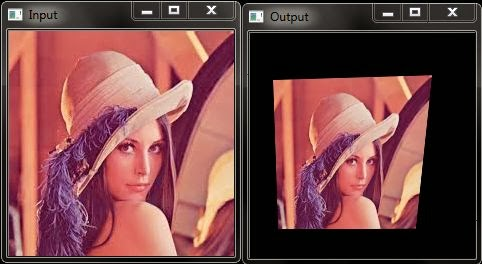
\includegraphics[width=0.5\textwidth]{imagens/Perspective_Transform.JPG}
    \caption{Resultado de uma transformação de perspectiva em uma imagem}
  \label{fig:perspectiva}
\end{figure}

\section{Identificando as marcações de notas}
\label{sec:ident_notas}

Partindo da imagem capturada da câmera do usuário, o programa procura
os marcadores dos cantos da folha, o código de barras e os interpreta
guardando as informações necessárias. Essas verificações acontecem a
cada frame capturado pela câmera para manter a integridade com a
imagem de tempo real. Com os pontos capturados a partir dos marcadores
é selecionada a área de interesse da folha que o programa deverá
interpretar ao sinal do usuário.

\begin{figure}[H]
  \centering
    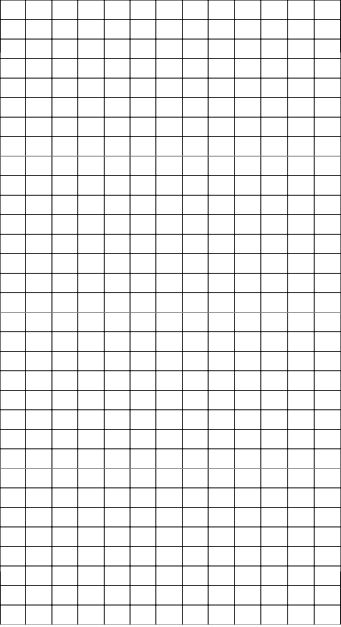
\includegraphics[angle=90,origin=c,width=0.5\textwidth]{imagens/aoi.png}
    \caption{Área central de uma folha}
  \label{fig:aoi_aoi}
\end{figure}

Com a informação de quantas colunas existem na área quadriculada,
adquirida do código de barras presente na folha, a próxima etapa
executada pelo algoritmo é de verificar em cada um dos retângulos da
área de interesse se há dois tipos de marcações diferentes: uma
representa um som que só tocará naquele momento e a outra representa a
continuidade do som, permitindo que ela seja reproduzido durante o
tempo desejado pelo usuário.

Foram escolhidas duas marcações diferentes para o software identificar
quando deve ocorrer cada uma das duas situações. O que identifica se a
nota será ou não mantida, é haver ou não pixels marcados do meio da
marcação original padrão até o final do quadrado identificado pelo
programa.

\begin{figure}[H]
  \centering
  \begin{subfigure}{0.4\textwidth}
    \centering
    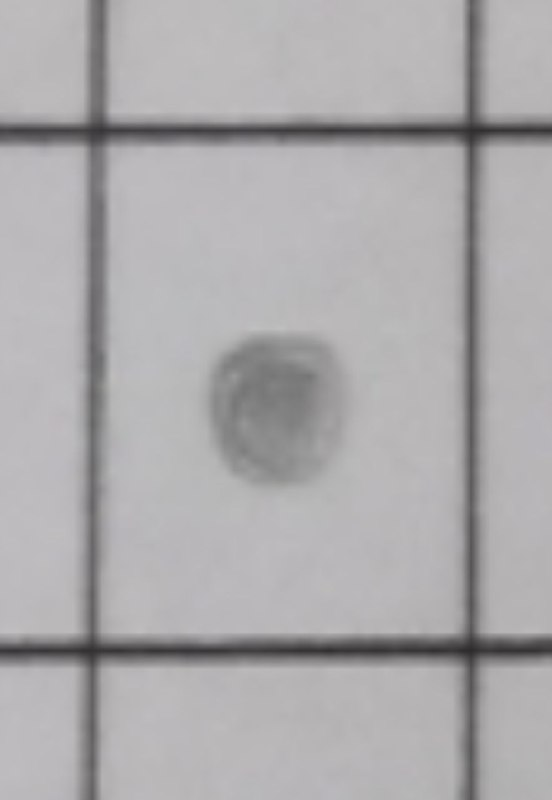
\includegraphics[width=0.4\textwidth]{imagens/nota.jpg}
    \caption{Marcação de nota}
    \label{fig:marcacao}
  \end{subfigure}
  %
  \begin{subfigure}{0.4\textwidth}
    \centering
    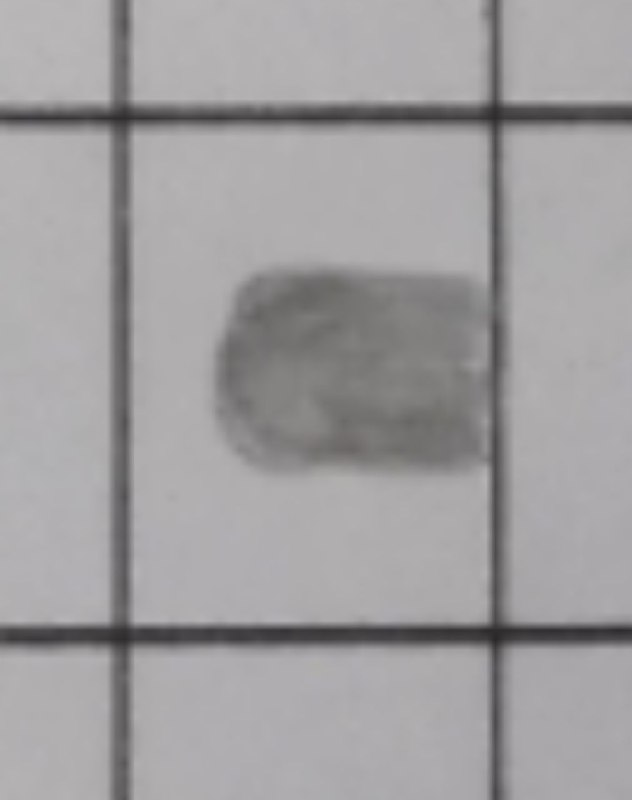
\includegraphics[width=0.4\textwidth]{imagens/nota_continuada.jpeg}
    \caption{Marcação de nota continuada}
    \label{fig:marcacao_continuada}
  \end{subfigure}%
\end{figure}

A partir das informações que o programa consegue da etapa anterior,
ele envia mensagens MIDI, utilizando o protocolo MIDI, para se
comunicar com uma fonte de áudio selecionada pelo usuário, a qual será
responsável pela reprodução dos sons em si. Isso tudo com um intervalo
de tempo definido entre cada nota, devido à cálculos a partir da
fórmula do compasso daquele modelo, extraída do código de barras da
folha, e definida ao gerar o pdf a partir de um segundo programa
criado para esse propósito.

Devido à falta de dinamicidade, uma vez que é impossível alterar
quantos retângulos existem na folha de papel após impressa, não foi
possível utilizar a fórmula de compasso convencional na teoria
musical, então foi definida uma convenção de que, para o software,
existem dois valores: um que determina quantas batidas aquela folha
comportará e outro que determina quantas notas serão tocadas em cada
batida.

Os cálculos feitos para se obter o tempo de coluna da folha é um
simples cálculo utilizando a fórmula do compasso convencionada e o
valor de batidas por minuto ($bpm$) passado como parâmetro, pelo usuário, ao
executar o software:

\begin{equation}
tempo = \dfrac{60}{bpm \times y}
\end{equation}

\noindent onde $y$ representa o número de sons que serão reproduzidos
a cada batida, ou seja, o denominador da fórmula do compasso
convencionada.

A ordem de disposição das notas foi escolhida da maneira como mostrada
na imagem \ref{fig:modelo_} pois é o mais próximo de como uma "pista"
MIDI é representada em {\it softwares} profissionais de gravação de
músicas, denominados DAW ({\it Digital Audio Workstation}), quando o
usuário utiliza recursos MIDI. A Figura \ref{fig:reaper} ilustra esse
conceito.

\begin{figure}[H]
  \centering
    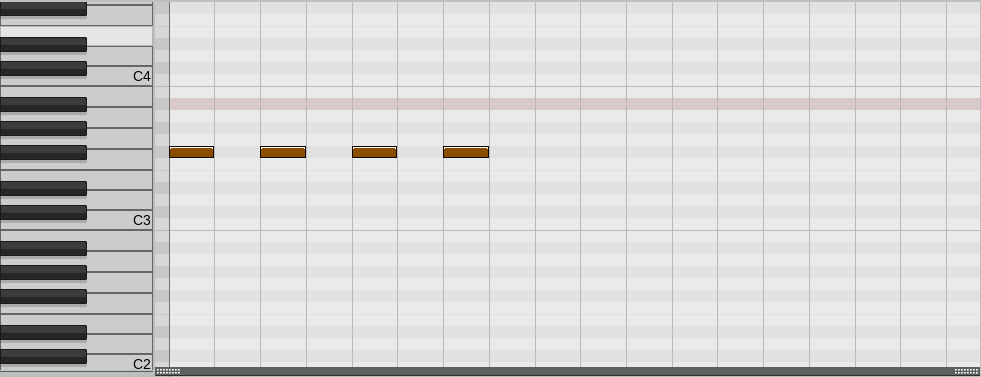
\includegraphics[width=0.5\textwidth]{imagens/midi_item_reaper.png}
    \caption{{\it Midi Item} na DAW Reaper}
  \label{fig:reaper}
\end{figure}

Também podemos interpretar o layout como um gráfico num simples plano
cartesiano. O gráfico representa $tempo \times frequência$, fazendo
com que a posição da marcação represente uma frequência num intervalo
de tempo. Essa interpretação pode ser representada da seguinte
maneira:

\begin{figure}[H]
  \centering
  \begin{subfigure}{0.4\textwidth}
    \centering
    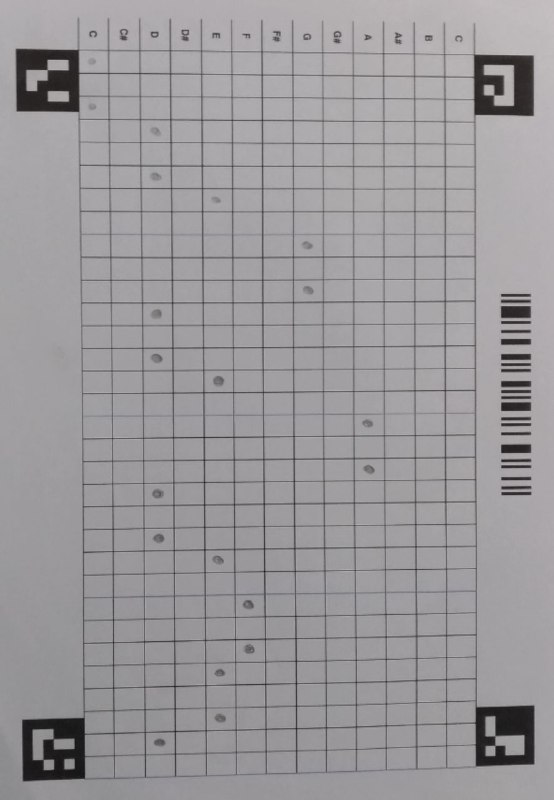
\includegraphics[angle=90,origin=c,width=1\textwidth]{imagens/layout_preenchido.jpeg}
    \caption{Folha com marcações}
    \label{fig:layout_marcacao}
  \end{subfigure}
  %
  \begin{subfigure}{0.5\textwidth}
    \centering
    \begin{tikzpicture}
      \begin{axis}
        [
          xlabel={$t$},
          ylabel={$f$},
          xmin=0, xmax=33,
          ymin=0, ymax=13,
        ]
        \addplot+[ycomb, domain=1:10, blue] table [x={n}, y={xn}] {data.dat};
      \end{axis}
    \end{tikzpicture}
    \caption{Gráfico discreto}
    \label{fig:gráfico}
  \end{subfigure}%
\end{figure}


% \begin{tikzpicture}
%   \begin{axis}
%     [
%       xlabel={$x$},
%       ylabel={$y$},
%       xmin=0, xmax=9,
%       ymin=0, ymax=13,
%     ]
%   \addplot+[ycomb, domain=1:10, blue] table [x={n}, y={xn}] {data.dat};
%   \end{axis}
% \end{tikzpicture}

\chapter{Resultados}
\label{cha:results}

Ao se iniciar o software, é necessário passar três parâmetros iniciais
na sua execução. O primeiro é o identificador da entrada de vídeo do
usuário para a cena ser capturada com a câmera correta caso haja mais
de uma conectada.

O segundo é a velocidade de batidas por minuto (bpm) para o tempo de
referência para reprodução das notas reproduzidas pelo software. Ao
gerar o modelo da folha, o usuário deve passar os valores que ditaram
a regra de velocidade de cada intervalo de tempo baseado no bpm
informado pelo usuário. Devido à limitações de espaço, o máximo de
retângulos que podem ser gerados para o bom funcionamento do software
é de 46 retângulos. Um exemplo que faria com que o software
apresentasse inconsistência pode ser encontrado abaixo:

\begin{figure}[H]
  \centering
    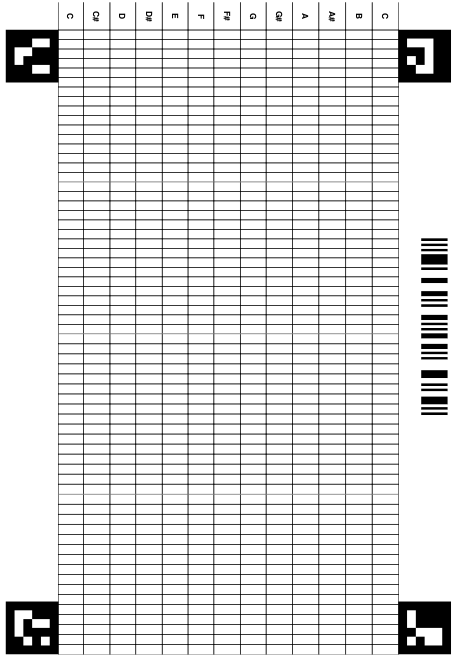
\includegraphics[angle=90,origin=c,width=0.4\textwidth]{imagens/416.png}
    \caption{Folha com 4 batidas por folha e 16 notas por batida}
  \label{fig:416}
\end{figure}

Podemos ver que, dependendo do que o usuário definisse, a espaço livre
para as marcações seria muito pequeno, prejudicando o funcionamento do
software, pelo menos em uma folha A4, onde se planejou originalmente o
uso da ferramenta. Folhas de dimensão maior podem atenuar esse
problema.

O terceiro é a oitava que será reproduzida no software. A oitava, na
teoria musical, representa uma nota com o dobro ou metade de sua
frequência. É quando a nota será, apesar de ter uma frequência maior
ou menor que a nota de referência, a mesma e se chama oitava devido ao
fato de, na representação mais comum das notas ({\bf dó, ré, mi, fá, sol,
lá, si}), ela seria a oitava nota, que seria a mesma da primeira porém
com uma frequência dobrada, ou seja: dó (oitava x), ré, mi, fá, sol,
lá, si e dó (oitava x+1), onde o último só e a oitava nota em relação
ao primeiro.

Com esses parâmetros definidos, o {\it software} inicia-se e lista
todas as entradas midi disponíveis no momento para o usuário escolher
a que o software enviará as mensagens do protocolo. Os parâmetros
iniciais informados pelo usuário ao iniciar o {\it software} são
apenas para configuração inicial do ambiente, porém, ao iniciar-se o
software de maneira correta, são editáveis a partir do clique de
teclas específicas informadas pelo programa.

Após essas configurações iniciais, é preciso se cumprir, assim como
outros softwares que utilizam conceitos de visão artificial, certas
condições para o funcionamento correto do software projetado neste
trabalho.

Primeiramente precisa-se de condições de ambiente favoráveis à captura
das imagens da câmera como iluminação da cena, principalmente de forma
que a folha não fique muito escura ou com sombreados escuros ou com
brilho excessivo, pois o filtro de branco utilizado na área de
interesse pode identificar sombras como marcações ou a inexistência
delas, o prejudica no funcionamento do software.

Outra condição é o posicionamento da câmera de forma que se consiga
visualizar os quatro marcadores ArUco e o código de barras presentes
na folha. Marcações serão mostradas no vídeo quando os cinco elementos
forem identificados de forma correta. Abaixo temos a imagem capturada
pela câmera com as devidas marcações indicando que as instruções
iniciais foram seguidas como o desejado:

\begin{figure}[H]
  \centering
    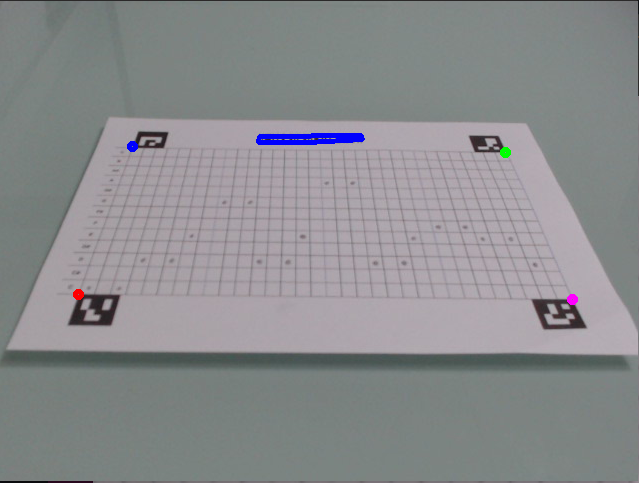
\includegraphics[width=0.4\textwidth]{imagens/video_com_marcacoes.png}
    \caption{Imagem capturada pela câmera com marcações de reconhecimento}
    \label{fig:tudo_ok}
\end{figure}

A partir desse ponto, pode-se utilizar a barra de espaço para o
software tocar ou parar a sequência identificada na folha. Essa
sequência pode ser livremente alterada pelo usuário diretamente na
folha de papel e reproduzida novamente quando se desejar, bastando
apenas que as condições já explicadas sejam sempre cumpridas antes de
se informar ao software que ele deverá reproduzir a sequência da
folha.

As marcações devem ser feitas sempre o mais centralizadas possível no
retângulo que indica o espaço de tempo da sequência, sendo possível
representar sons que vão continuar soando ou que vão parar no próximo
intervalo de tempo com duas marcações distintas já mostradas no
capítulo que destrincha o algoritmo utilizado.

Os valores que podem ser alterados durante a execução do software,
diretamente no próprio software controlador, e não no sintetizador,
são o valores do bpm e da oitava, além de indicadores para determinar
se haverá {\it stop} ou {\it play} ao se pressionar a barra de espaço
e para determinar se o software enviará mensagens para o canal dez,
que simula instrumentos de percussão, ou para o canal um que simula
instrumentos melódicos. As teclas responsáveis para somar e subtrair
desses valores, respectivamente, são seta para cima, seta para baixo,
seta para direita e seta para esquerda. Para ativar ou desativar o
modo de bateria, a tecla correspondente é a tecla M do teclado.

Quando em ambiente bem iluminada e a câmera se encontra corretamente
ajustada e marcações devidamente adicionadas à folha, o software
apresenta ótimos resultados em conjunto com softwares sintetizadores
que seguem o Protocolo MIDI, pecando apenas na temporização das notas
devido ao algoritmo utilizado.

Também é possível utilizar o software como um controlador midi em uma
DAW, porém, da forma como ele está no momento da escrita desde
documento, ainda apresenta inconsistências quando utilizada dessa
forma. A DAW utilizada para se obterem os resultados chama-se Reaper e
é gratuita.

Pode-se considerar, de certa forma, cada folha de papel como um
compasso de uma partitura musical, o torna possível a composição não
de músicas completas, mas sim de trechos e ideias de músicas, e o
usuário pode guardá-las assim como se faz com partituras, tablaturas e
gravações, porém com a vantagem de alterar o tempo e o instrumento a
cada vez que reproduzir a informação contida na folha de papel.

\chapter{Conclusões}
\label{cha:conclusoes}

O software desenvolvido consiste num algoritmo criado especificamente
para o que o software pretende entregar para o usuário. Utilizando de
conceitos de visão artificial e de comunicação MIDI para interpretar
informações e elementos, a partir de uma folha A4 impressa com um
layout específico e preenchida de acordo com o que o usuário pretende
que seja reproduzido, e enviando mensagens MIDI para um segundo
software sintetizador escolhido elo usuário, que será o responsável
por reproduzir as notas desejadas e encontradas na folha de papel.

Durante o desenvolvimento, foi preciso armazenar informações no modelo
da folha de papel e se identificar pontos distintos para haver uma
transformada de perspectiva na imagem original capturada pela câmera
e, para esses dois quesitos, foram utilizados como solução um código
de barras para o armazenamento das informações e marcadores ArUco para
o software determinar corretamente a área de maior interesse da folha.

Devido à reprodução e repetição do algoritmo não otimizado de maneira
correta, o software acaba tendo problemas com relação à temporização
de cada nota, para a qual foi convencionado um substituto da fórmula
do compasso da teoria musical para ser aplicado um cálculo de tempo
que cada nota deve ser mantida ativada. Uma solução seria a aplicação
de um vetor de mensagens MIDI que seria preenchido no momento que o
software interpretasse folha de papel da primeira vez e com isso, ao
invés do software procurar informação em cada retângulo da folha a
todo momento, o que gera {\it overhead} considerável.

Isso só aconteceria à leitura desse vetor onde foram armazenadas as
mensagens MIDI, tornando o programa mais veloz e provavelmente
solucionando o problema da temporização de cada som e adicionando
também a possibilidade de serem criados diferentes vetores a partir de
diferentes folhas de papel. Essa funcionalidade poderia tornar
possível o usuário reproduzir mais de uma folha de papel em sequência.

O software utiliza interfaces para o usuário disponibilizadas pela
biblioteca de visão artificial OpenCV, porém essas interfaces não são
modernas ou intuitivas, prejudicando a experiência do usuário
final.

Outra adição ao programa seria criar uma interface visual intuitiva e
moderna com as opções de se selecionar a oitava, velocidade, volume,
instrumento que o sintetizador deverá simular, criar um novo pdf a
partir de parâmetros definidos do usuário diretamente da aplicação e
não utilizando um segundo programa e uma visualização, no caso da
adição da funcionalidade dos vetores apresentada no parágrafo
anterior, de cada folha de papel armazenada e uma linha do tempo de
qual folha está sendo reproduzida no momento caso o usuário tenha
escolhido reproduzir mais de uma folha em sequência.

Ressalte-se que a ferramenta criada apresenta grande potencial também
para o ensino de teoria musical, pois é capaz de ilustrar para os
alunos o conceito de altura, tempo de duração de notas, bem como o
ritmo, utilizando recursos de baixíssimo custo e altamente interativos.

\appendix
\chapter{Biblioteca RtMidi}

O sintetizador escolhido pelo usuário precisa receber as mensagens
enviadas pelo software e foi com auxílio da biblioteca RtMidi para a
linguagem de programação C++ que foi possível abstrair todo o fluxo de
troca de mensagens em simples funções disponibilizadas pela
biblioteca.

Para a utilização do protocolo MIDI e para a comunicação entre
sintetizadores, foi escolhida a biblioteca RtMidi para a linguagem de
programação C++. Toda a transmissão e criação das mensagens foi
abstraída durante o desenvolvimento do projeto graças às
funcionalidades da biblioteca e foi por esse motivo, além de ser Open
Source, que ela foi escolhida para fazer parte do desenvolvimento do
software.

A biblioteca consiste em duas classes chamadas RtMidiOut e RtMidiIn. A
classe RtMidiOut proporciona, para o desenvolvedor, funcionalidades
simples para a imediata troca de mensagens MIDI entre dispositivos
virtuais ou não conectados através de uma conexão MIDI. Com essas
funcionalidades foi possível ocorrer o envio de mensagens para o
sintetizador selecionado pelo usuário como porta de entrada ou cliente
para escrita da conexão midi com apenas o uso, após configurada essa
entrada, de uma função responsável exclusivamente pelo envio dessas
mensagens.

A outra classe, RtMidiIn, apesar de não ter sido utilizada no software
apresentado neste trabalho, utiliza uma função interna de callback ou
thread para receber mensagens MIDI que são enviadas a partir de uma
porta de saída MIDI selecionável e as lendo, transformando no formato
utilizado pela biblioteca, ou repassando-a imediatamente para uma
função de callback especificada pelo usuário, o que tornaria possível,
por exemplo, o software reproduzir, num sintetizador digital, o que
foi enviado a partir de um controlador físico conectado à máquina do
usuário.

Ao se instanciar um objeto da classe RtMidiOut, é criada uma saída
virtual MIDI a qual pode se comunicar com qualquer entrada midi
disponível e, ao se instanciar um objeto da classe RtMidiIn, é criada
uma entrada midi virtual e essa pode receber mensagens de qualquer
saída midi disponível, desde de que haja conexão entra as saídas e
entradas que se deseja.

Um exemplo, utilizado na documentação da biblioteca \cite{rtmidi}, de aplicação da classe RtMidiOut pode ser visto abaixo:

\begin{lstlisting}
// midiout.cpp
#include <iostream>
#include <cstdlib>
#include "RtMidi.h"
int main()
{
  RtMidiOut *midiout = new RtMidiOut();
  std::vector<unsigned char> message;
  // Check available ports.
  unsigned int nPorts = midiout->getPortCount();
  if ( nPorts == 0 ) {
    std::cout << "No ports available!\n";
    goto cleanup;
  }
  // Open first available port.
  midiout->openPort( 0 );
  // Send out a series of MIDI messages.
  // Program change: 192, 5
  message.push_back( 192 );
  message.push_back( 5 );
  midiout->sendMessage( &message );
  // Control Change: 176, 7, 100 (volume)
  message[0] = 176;
  message[1] = 7;
  message.push_back( 100 );
  midiout->sendMessage( &message );
  // Note On: 144, 64, 90
  message[0] = 144;
  message[1] = 64;
  message[2] = 90;
  midiout->sendMessage( &message );
  SLEEP( 500 ); // Platform-dependent ... see example in tests directory.
  // Note Off: 128, 64, 40
  message[0] = 128;
  message[1] = 64;
  message[2] = 40;
  midiout->sendMessage( &message );
  // Clean up
 cleanup:
  delete midiout;
  return 0;
}
\end{lstlisting}

O exemplo apresentado da documentação oficial para a classe RtMidiIn pode ser visualizado logo a seguir:

\begin{lstlisting}
// qmidiin.cpp
#include <iostream>
#include <cstdlib>
#include <signal.h>
#include "RtMidi.h"
bool done;
static void finish(int ignore){ done = true; }
int main()
{
  RtMidiIn *midiin = new RtMidiIn();
  std::vector<unsigned char> message;
  int nBytes, i;
  double stamp;
  // Check available ports.
  unsigned int nPorts = midiin->getPortCount();
  if ( nPorts == 0 ) {
    std::cout << "No ports available!\n";
    goto cleanup;
  }
  midiin->openPort( 0 );
  // Don't ignore sysex, timing, or active sensing messages.
  midiin->ignoreTypes( false, false, false );
  // Install an interrupt handler function.
  done = false;
  (void) signal(SIGINT, finish);
  // Periodically check input queue.
  std::cout << "Reading MIDI from port ... quit with Ctrl-C.\n";
  while ( !done ) {
    stamp = midiin->getMessage( &message );
    nBytes = message.size();
    for ( i=0; i<nBytes; i++ )
      std::cout << "Byte " << i << " = " << (int)message[i] << ", ";
    if ( nBytes > 0 )
      std::cout << "stamp = " << stamp << std::endl;
    // Sleep for 10 milliseconds ... platform-dependent.
    SLEEP( 10 );
  }
  // Clean up
 cleanup:
  delete midiin;
  return 0;
}
\end{lstlisting}

Para o testes do software, foram utilizados 3 softwares de terceiros,
sendo eles o QSynth, sintetizador virtual MIDI, o VMPK, outro
sintetizador virtual MIDI mas também controlador, e o QJackCtl, um
software que permite o usuário administrar as conexões MIDI entre
saídas e entradas MIDI disponíveis na máquina.

Abaixo pode-se visualizar como se dá a comunicação dos softwares
controlador e sintetizador:

\begin{figure}[H]
  \centering
  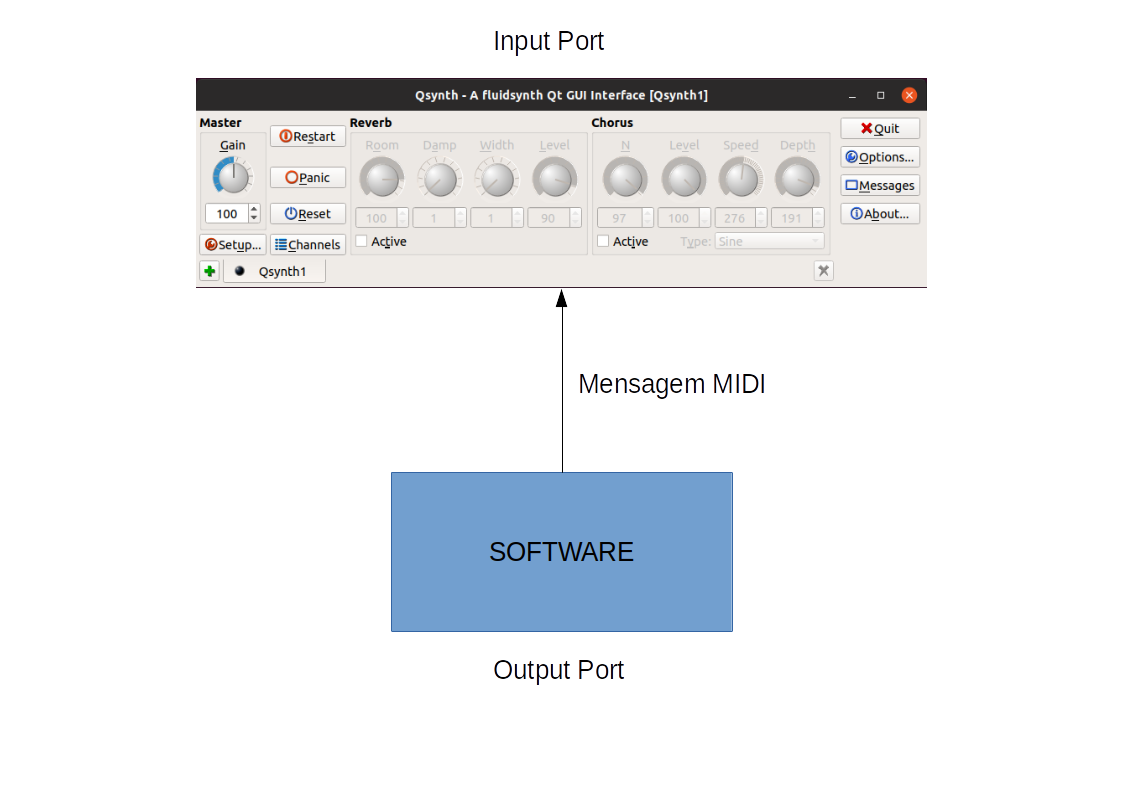
\includegraphics[width=1\textwidth]{imagens/Diagrama2.png}
  \caption{Diagrama de fluxo entrada e saída MIDI}
  \label{fig:diagrama}
\end{figure}

\noindent onde as portas de saída são os controladores e as de entrada
são os sintetizadores.



\chapter{Passo-a-passo para utilização do software}
A utilização do software consiste em alguns passos que devem ser
seguidos para seu funcionamento.

Primeiramente é necessário gerar um modelo de folha de papel a partir
de um software secundário que recebe os parâmetros da fórmula do
compasso convencionada no desenvolvimento do software que utiliza
visão artificial. Esses parâmetros são o número de batidas por folha e
quantas notas serão tocadas a cada batida do bpm selecionado pelo
usuário na execução do software primário. Pode-se perceber, nos
modelos abaixo, que há uma divisão em cinza para cada batida do bpm, o
que indica de forma visual qual foi a composição utilizada na geração
do modelo.

\begin{figure}[H]
  \centering
  \begin{subfigure}{0.4\textwidth}
    \centering
    \includegraphics[angle=90,origin=c,width=0.9\textwidth]{imagens/modelo44.png}
    \caption{Modelo com 4 batidas por folha e 4 notas por batida}
    \label{fig:modelo44}
  \end{subfigure}
  %
  \begin{subfigure}{0.4\textwidth}
    \centering
    \includegraphics[angle=90,origin=c,width=0.9\textwidth]{imagens/modelo48.png}
    \caption{Modelo com 4 batidas por folha e 8 notas por batida}
    \label{fig:modelo48}
  \end{subfigure}
\end{figure}

  %
\begin{figure}[H]
  \centering
  \begin{subfigure}{0.4\textwidth}
    \centering
    \includegraphics[angle=90,origin=c,width=0.9\textwidth]{imagens/modelo84.png}
    \caption{Modelo com 8 batidas por folha e 4 notas por batida}
    \label{fig:modelo84}
  \end{subfigure}
  %
  \begin{subfigure}{0.4\textwidth}
    \centering
    \includegraphics[angle=90,origin=c,width=0.9\textwidth]{imagens/modelo162.png}
    \caption{Modelo com 16 batidas por folha e 2 notas por batida}
    \label{fig:modelo162}
  \end{subfigure}
\end{figure}

Onde podemos comparar, levando um compasso de uma partitura como
referência, o modelo da figura \ref{fig:modelo44} com um compasso de
uma partitura com, no máximo, dezesseis semicolcheias, o modelo da
figura \ref{fig:modelo48} com um compasso com, no máximo, 32 fusas, o
modelo da figura \ref{fig:modelo84} com um compasso com, no máximo, 32
semicolcheias e o modelo da figura \ref{fig:modelo162} com um compasso
com, no máximo, 32 colcheias, sendo possível, devido à implementação
da identificação de marcação de nota continuada, mostrada na figura
\ref{fig:marcacao_continuada}, utilizar notas que fiquem ativas
durante mais de um intervalo de tempo da folha.

Abaixo há uma referência para a nomenclatura das figuras de tempo, utilizadas no parágrafo anterior:

\begin{figure}[H]
  \centering
  \begin{subfigure}{0.4\textwidth}
    \centering
    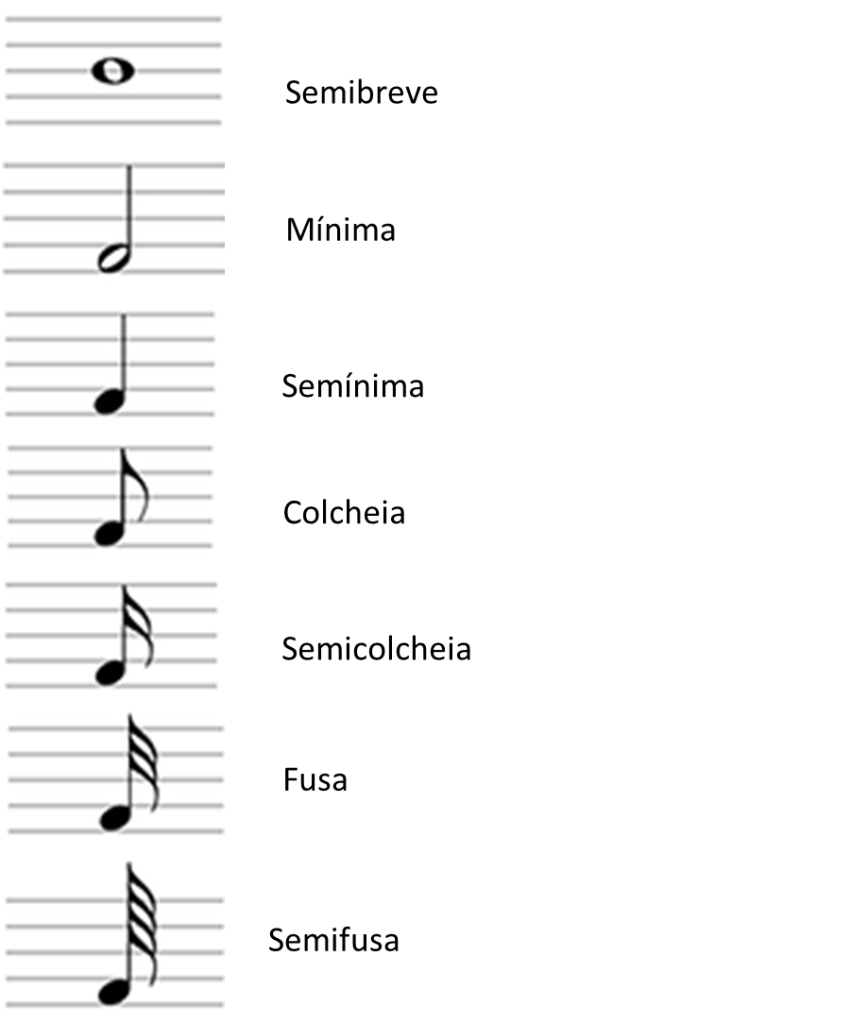
\includegraphics[width=0.8\textwidth]{imagens/tempos.png}
    \caption{Figuras musicais para representação de tempo}
    \label{fig:tempos}
  \end{subfigure}
  %
  \begin{subfigure}{0.4\textwidth}
    \centering
    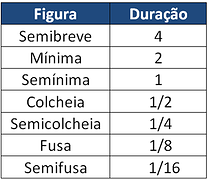
\includegraphics[width=0.8\textwidth]{imagens/semibreve.png}
    \caption{Valores de cada figura}
    \label{fig:tempos_valores}
  \end{subfigure}
\end{figure}

Com a folha impressa, inicia-se o software primário com os parâmetros
que representam, respectivamente, o identificador da câmera que o
usuário utilizará para capturar as imagens, o bpm que será levado como
referência no cálculo do tempo de cada nota e a oitava, indicando
quais valores o conjunto de 13 sons representarão no
sintetizador. Após a iniciação correta do software, o usuário deverá
informar, dentro as entradas listadas, qual ele quer que receba as
mensagens enviadas pelo programa.

Após serem definidos os parâmetros de inicialização, o usuário deve
posicionar a folha de papel de maneira que a câmera identifique ambos
os quatro marcadores ArUco tanto o código de barras. No momento que
forem interpretados da maneira correta, marcadores aparecerão na tela
indicando que o usuário pode prosseguir normalmente.

%Ver figura \ref{tudo_ok}.

Após os elementos serem devidamente interpretados pelo software, uma
nova janela aparecerá e nela estará a área de interesse da folha com a
transformada de perspectiva aplicada para melhor visualização das
marcações tanto para o usuário quanto para o próprio software. Após
isso, usuário poderá pressionar barra de espaço para o programa
começar a enviar as mensagens midi, correspondentes às marcações
presentes na folha, para o sintetizador. Para cada coluna lida pelo
software, uma marcação é adicionada à imagem transformada,
representando qual coluna o software está lendo no momento, como
apresentado na figura abaixo:

\begin{figure}[H]
  \centering
  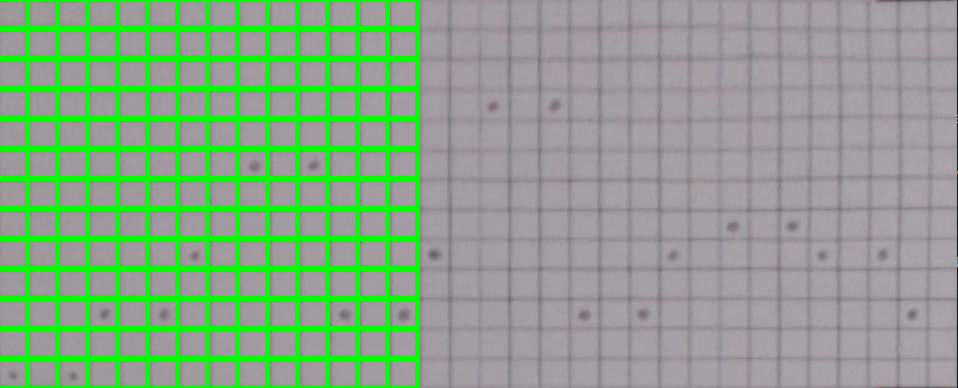
\includegraphics[width=1\textwidth]{imagens/area_transformada_preenchida.png}
  \caption{Indicações de qual coluna está sendo interpretada no momento}
  \label{fig:colunas_marcacoes}
\end{figure}

Abaixo é possível visualizar uma folha com os quatro primeiros
compassos da música "Dó Ré Mi Fá". Cada folha representaria apenas um
compasso por vez da música original, porém, devido à solução
encontrada para essa limitação, que é a fórmula do compasso
convencionada já discuta anteriormente, é possível reproduzir quatro
compassos em uma única folha, como é possível de se visualizar
abaixo. A folha em questão possui os seguintes parâmetros: 16 e 2, os
quais fazem cada batida representar uma coluna da folha, ou seja, 16
batidas por folha, duas notas por batida e 32 notas ou conjunto de
notas por folha, a qual, quando comparada a um compasso de uma
partitura, pode-se dizer que representa um compasso com no máximo 32
colcheias.

\begin{figure}[H]
  \centering
  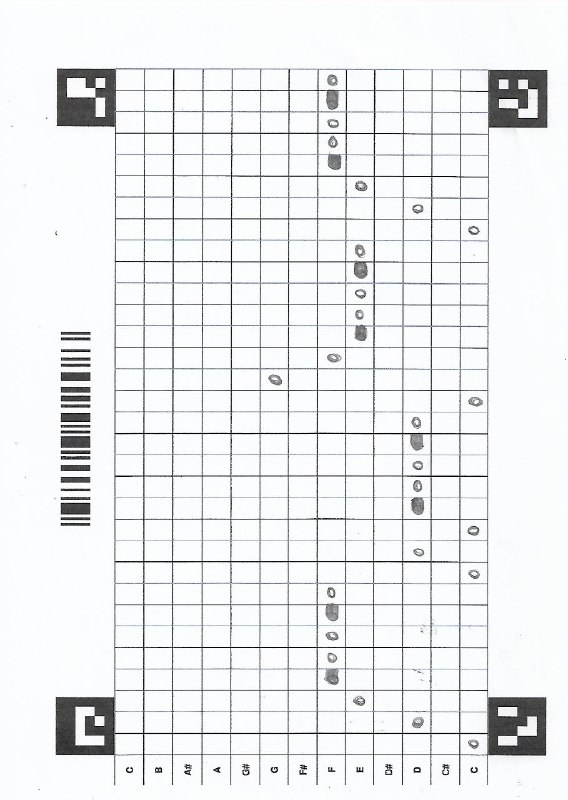
\includegraphics[angle=270,origin=c,width=1\textwidth]{imagens/doremifa.jpeg}
  \caption{Folha que simula a música "Dó Ré Mi Fá"}
  \label{fig:doremifa}
\end{figure}

Também é possível, com o modo de bateria ativado, ao se pressionar a
tecla M, reproduzir acompanhamentos de bateria em sequência. A figura
abaixo representa uma bateria de rock, onde se tem dois bumbos em
sequência seguidos por uma caixa com acompanhamento de chimbal:

\begin{figure}[H]
  \centering
  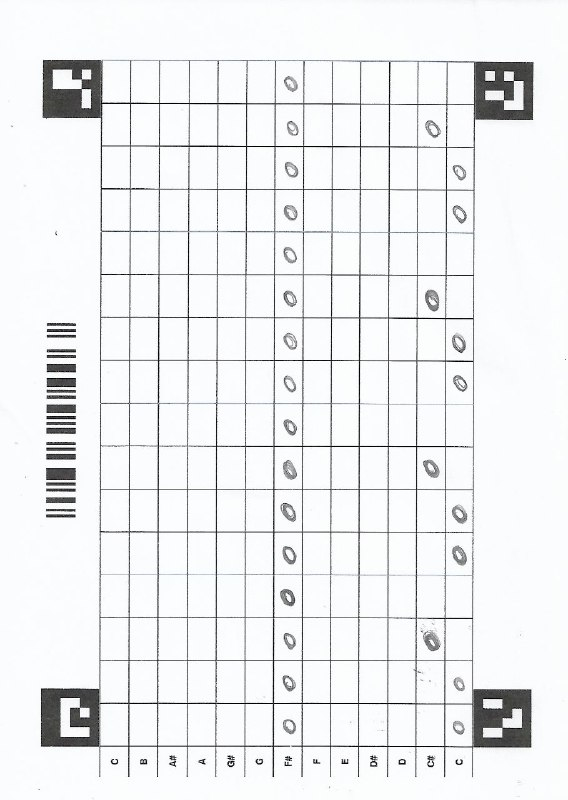
\includegraphics[angle=270,origin=c,width=1\textwidth]{imagens/bateria_rock.jpeg}
  \caption{Folha que simula um ritmo de rock}
  \label{fig:bateria_rock}
\end{figure}

\bibliography{referencias}

\end{document}
